\documentclass[tikz,border=10pt]{standalone}
\usetikzlibrary{arrows.meta}

\begin{document}
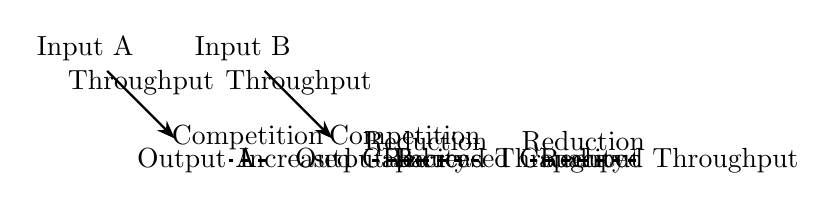
\begin{tikzpicture}[node distance=2cm]
    % Nodes for inputs and outputs
    \node (inputA) {Input A};
    \node (outputA) [below right of=inputA] {Output A};
    \node (inputB) [right of=inputA] {Input B};
    \node (outputB) [below right of=inputB] {Output B};

    % Arrows from inputs to outputs
    \draw[-Stealth, thick] (inputA) -- node[above] {Throughput} (outputA);
    \draw[-Stealth, thick] (inputB) -- node[above] {Throughput} (outputB);

    % Nodes for capacity increases
    \node (capacityA) [right of=outputA] {Increased Capacity};
    \node (capacityB) [right of=outputB] {Increased Capacity};

    % Arrows showing competition
    \draw[dashed, thick] (outputA) -- node[midway, above] {Competition} (capacityA);
    \draw[dashed, thick] (outputB) -- node[midway, above] {Competition} (capacityB);

    % Nodes for reduced throughput
    \node (reducedA) [right of=capacityA] {Reduced Throughput};
    \node (reducedB) [right of=capacityB] {Reduced Throughput};

    % Arrows showing reduced throughput
    \draw[dashed, thick] (capacityA) -- node[midway, above] {Reduction} (reducedA);
    \draw[dashed, thick] (capacityB) -- node[midway, above] {Reduction} (reducedB);
\end{tikzpicture}
\end{document}